% !TeX program = xelatex
% !TeX encoding = UTF-8
% !TeX TXS-program:compile = txs:///xelatex | txs:///xelatex
\documentclass[aspectratio=169, table, 12pt]{beamer}

% Preamble bersama seluruh slide mata kuliah ini.
% Dipanggil dari slides/sessionXX/sessionXX.tex tepat sesudah baris
% \documentclass[aspectratio=169, table, 12pt]{beamer}
% Paket tambahan yang hanya dibutuhkan satu sesi ditulis di berkas sesi itu.

\usepackage{colortbl}
\usepackage{xcolor}
\usepackage{listings}
\usepackage{tabularx}
\usepackage{booktabs}
\usepackage{tikz}
\usepackage{pgfplots}
\usepackage{fontspec}
\usepackage[english,bahasai]{babel}
\pgfplotsset{compat=1.18}
\usetikzlibrary{arrows.meta, positioning, calc, fit, shapes.geometric,
  shapes.multipart, backgrounds, matrix, chains, trees}

\makeatletter
\def\input@path{{../theme/}}
\makeatother
\graphicspath{{../theme/}{../../figures/}}
% Stub symlink Windows memakai tema cadangan sampai aset institusi tersedia.
\IfFileExists{../theme/beamerthemePradita.sty}{%
  \usetheme{Pradita}
}{%
  \usetheme{Madrid}
  \setmainfont{TeX Gyre Heros}
  \setsansfont{TeX Gyre Heros}
  \setbeamertemplate{navigation symbols}{}
}

\definecolor{praditagreen}{RGB}{37, 113, 71}
\setbeamercolor{structure}{fg=praditagreen}
\setbeamercolor{palette primary}{bg=praditagreen,fg=white}
\setbeamercolor{palette secondary}{bg=praditagreen!80!black,fg=white}
\setbeamercolor{palette tertiary}{bg=praditagreen!60!black,fg=white}
\setbeamerfont{frametitle}{size=\large}
\setbeamertemplate{caption}[numbered]

% Ukuran header mengikuti teks agar judul panjang tidak menabrak logo.
\setbeamercolor{frametitle}{bg=white,fg=black}
\setbeamertemplate{frametitle}{%
  \begin{beamercolorbox}[wd=\paperwidth,sep=0.2cm]{frametitle}
    \begin{minipage}[c]{0.77\paperwidth}
      \raggedright\fontsize{16}{18}\selectfont\bfseries\insertframetitle
      \ifx\insertframesubtitle\empty\else
        \par\small\mdseries\insertframesubtitle
      \fi
    \end{minipage}\hfill
    \begin{minipage}[c]{0.15\paperwidth}
      \IfFileExists{../theme/classFiles/logo_universitas.png}{%
        
\includegraphics[width=\linewidth]{../theme/classFiles/logo_universitas.png}%
      }{}
    \end{minipage}
  \end{beamercolorbox}
}
\setbeamertemplate{footline}{%
  \ifnum\value{framenumber}>1
    \begin{beamercolorbox}[wd=\paperwidth,ht=0.35cm,dp=0.15cm,
      leftskip=0.3cm,rightskip=0.3cm]{palette primary}
      \footnotesize\bfseries\insertframenumber/\inserttotalframenumber
      \hfill IT40813
    \end{beamercolorbox}
  \fi
}
\DeclareRobustCommand{\berkas}[1]{\path{#1}}

% Tema membuat garis tabel berwarna putih. Dikembalikan agar tabel terbaca.
\arrayrulecolor{black}
\setlength{\arrayrulewidth}{0.5pt}

\lstdefinelanguage{yaml}{
  basicstyle=\ttfamily\scriptsize,
  keywordstyle=\color{blue}\bfseries,
  commentstyle=\color{gray}\itshape,
  stringstyle=\color{red},
  showstringspaces=false,
  breaklines=true,
  frame=lines,
  numbers=none,
  backgroundcolor=\color{lightgray!10},
  tabsize=2,
  morecomment=[l]{\#}
}

\lstdefinelanguage{json}{
  basicstyle=\ttfamily\scriptsize,
  stringstyle=\color{red},
  commentstyle=\color{gray},
  breaklines=true,
  showstringspaces=false,
  tabsize=2,
  numbers=none,
  frame=lines,
  backgroundcolor=\color{lightgray!10},
  string=[s]{"}{"}
}

\lstdefinelanguage{bash}{
  keywords={},
  basicstyle=\ttfamily\scriptsize,
  ndkeywords={docker, kubectl, helm, curl, git, terraform},
  ndkeywordstyle=\color{purple}\bfseries,
  sensitive=true,
  commentstyle=\color{gray},
  numbers=none,
  breaklines=true,
  frame=lines,
  backgroundcolor=\color{lightgray!10},
  tabsize=2,
  comment=[l]{\#},
  showstringspaces=false
}

\lstdefinelanguage{http}{
  keywords={GET, POST, PUT, PATCH, DELETE, HEAD, OPTIONS, HTTP},
  basicstyle=\ttfamily\scriptsize,
  keywordstyle=\color{blue}\bfseries,
  sensitive=true,
  numbers=none,
  breaklines=true,
  frame=lines,
  backgroundcolor=\color{lightgray!10},
  tabsize=2,
  showstringspaces=false
}

\subtitle{IT40813 · IT Governance, Risk \& Compliance}
\author{\textbf{Alfa Yohannis}}


% Sampul membatasi judul di panel putih tema rujukan Pradita.
\setbeamertemplate{title page}{%
  \begin{tikzpicture}[remember picture,overlay]
    \node[anchor=north west,inner sep=0pt,text width=8.8cm]
      at ([xshift=1cm,yshift=-3.15cm]current page.north west) {%
        {\small\insertsubtitle\par}\vspace{0.25cm}
        \resizebox{8.8cm}{!}{\begin{minipage}{12cm}
          \raggedright\color{praditagreen}\bfseries\inserttitle
        \end{minipage}}
      };
    \node[anchor=south west,inner sep=0pt]
      at ([xshift=1cm,yshift=1.65cm]current page.south west)
      {\small\insertdate};
    \node[anchor=west,inner sep=0pt,text=white]
      at ([xshift=0.8cm,yshift=0.75cm]current page.south west)
      {\small\insertauthor};
  \end{tikzpicture}
}


\title{\Huge Alat GRC dan Peta Jalan\\ \vspace{10pt} Tata Kelola Terpadu}
\date{Pertemuan 14}

\begin{document}

\frame{\titlepage}

\begin{frame}
  \frametitle{Isi Pertemuan}
  \vspace{14pt}
  \begin{columns}[t]
    \column{0.5\textwidth}
    {\small\tableofcontents[sections={1-4}]}

    \column{0.5\textwidth}
    {\small\tableofcontents[sections={5-8}]}
  \end{columns}
\end{frame}

\begin{frame}{\hfill}
  \centering
  \Huge{\textbf{Semua angka benar\\di babnya masing-masing.\\Apakah semuanya muat\\dalam Rp10 miliar?}}
\end{frame}

\section{Tujuan dan Konteks}

\begin{frame}{{\Large Tujuan Pembelajaran}}
  \vspace{10pt}
  \begin{itemize}
    \item Membandingkan pilihan alat GRC, dari spreadsheet sampai platform terintegrasi, berdasarkan
          kebutuhan dan kematangan organisasi.
    \item Menyusun peta jalan GRC bertahap yang selaras dengan peta jalan transformasi digital.
    \item Mempertahankan rekomendasi tata kelola, risiko, dan kepatuhan di depan pemangku
          kepentingan.
  \end{itemize}
\end{frame}

\begin{frame}{{\Large Masalah: 20 Spreadsheet, Banyak Versi}}
  \vspace{6pt}
  \small
  \begin{itemize}
    \item Misalkan register risiko, kepatuhan, dan temuan audit tersimpan dalam 20 spreadsheet.
    \item Satu akun vendor dicatat sebagai tiga masalah dengan pemilik berbeda.
    \item Unit TI melaporkan 108 dari 108 akun, padahal populasinya 120 akun.
    \item Bab 1 sampai Bab 13 menghasilkan angka yang belum pernah dijumlahkan.
    \item Hasil kerja: peta jalan tiga tahun, pilihan alat, dan paket keputusan C4.
  \end{itemize}
\end{frame}

\begin{frame}{{\Large Alur Keputusan Bab Ini}}
  \vspace{20pt}
  \begin{center}
    \resizebox{0.95\textwidth}{!}{\begin{tikzpicture}[node distance=4mm, kotak/.style={draw, rounded corners, align=center, text width=1.85cm, minimum height=1.2cm, font=\scriptsize}, panah/.style={-{Stealth[length=2mm]}, thick}]
  \node[kotak,fill=praditagreen!15] (t0) {Risiko dan kewajiban};
  \node[kotak,fill=blue!8] (t1) [right=of t0] {Kontrol dan bukti bersama};
  \node[kotak,fill=blue!8] (t2) [right=of t1] {Alat sesuai kebutuhan};
  \node[kotak,fill=orange!12] (t3) [right=of t2] {Gelombang inisiatif};
  \node[kotak,fill=green!10] (t4) [right=of t3] {Keputusan dan asurans};
  \draw[panah] (t0) -- (t1);
  \draw[panah] (t1) -- (t2);
  \draw[panah] (t2) -- (t3);
  \draw[panah] (t3) -- (t4);
\end{tikzpicture}
}
  \end{center}
  \vspace{10pt}
  \small Seluruh angka, pemetaan, dan anggaran Medikara merupakan pengandaian pembelajaran.
\end{frame}

\begin{frame}{{\Large Diagram Konsep Bab 14}}
  \centering
  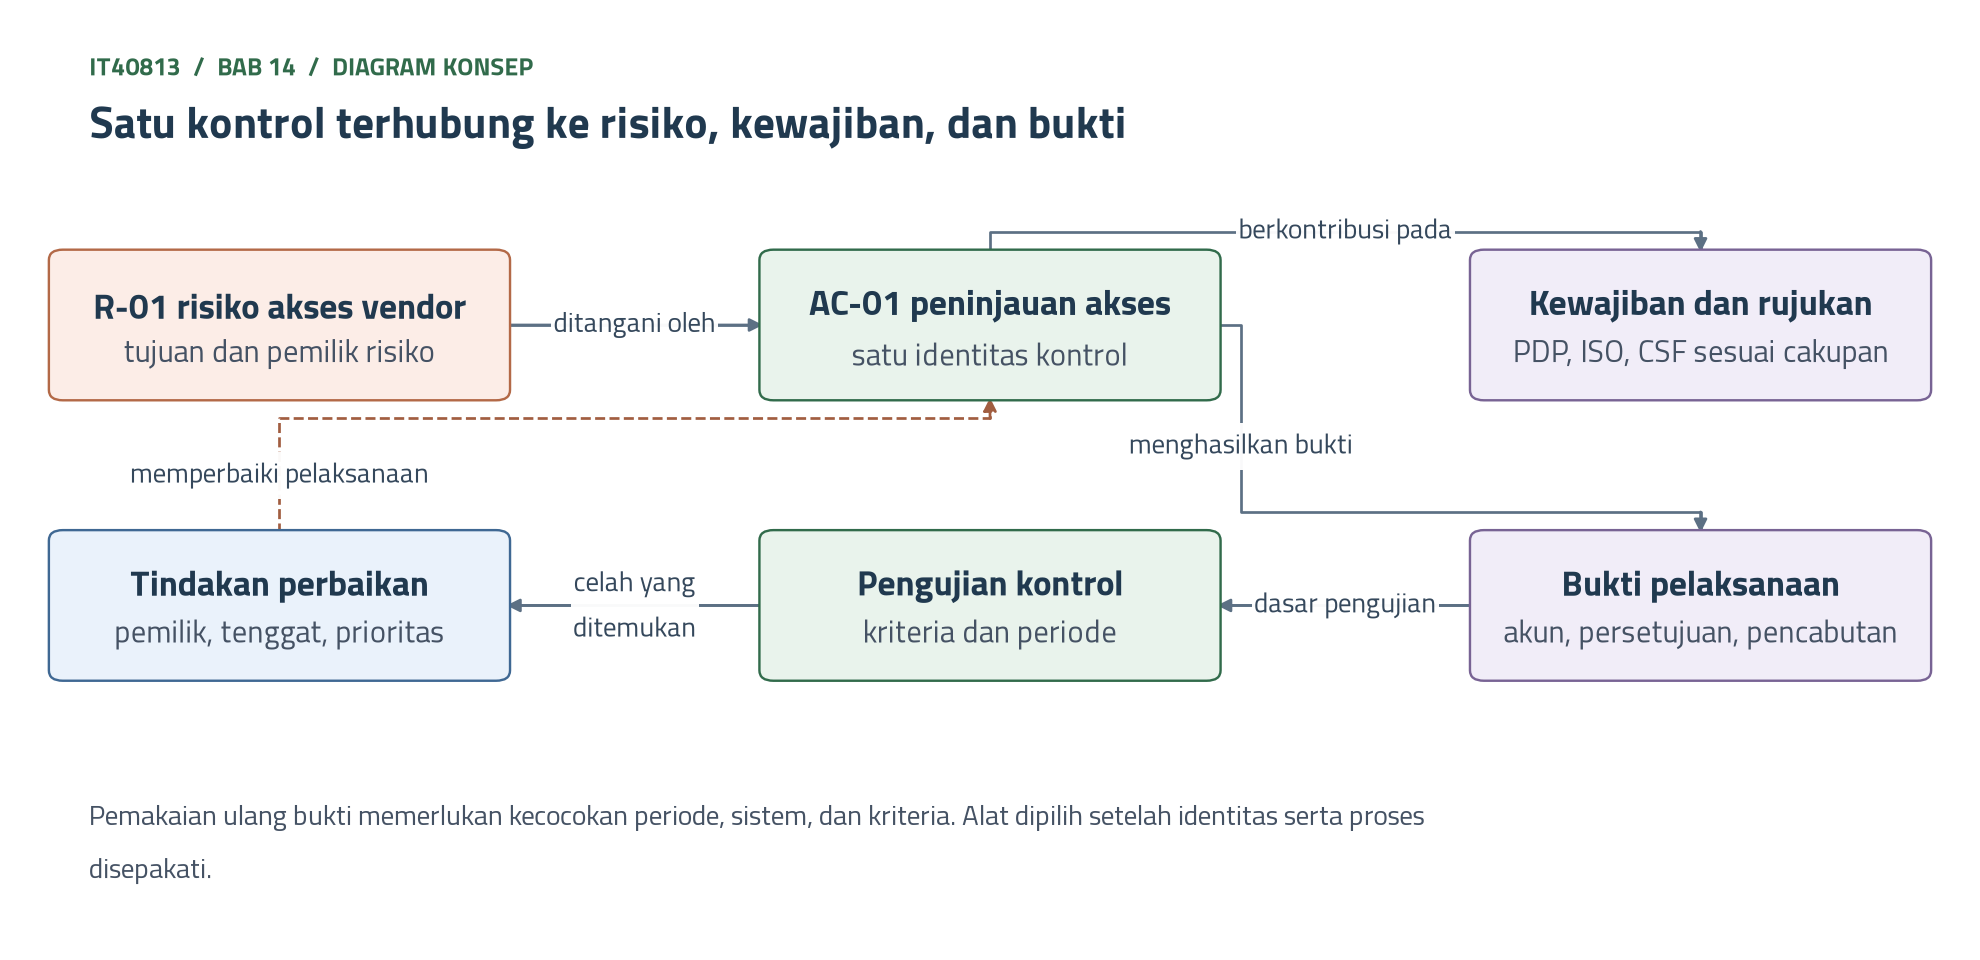
\includegraphics[width=0.96\textwidth,height=0.77\textheight,keepaspectratio]{../../figures/ch14-diagram-konsep.png}
  \label{fig:session14-ilustrasi-bab}
\end{frame}

\section{GRC Terpadu}

\begin{frame}{{\Large Satu Identitas untuk Satu Objek}}
  \vspace{6pt}
  \small
  \begin{itemize}
    \item GRC terpadu menghubungkan tujuan, risiko, kewajiban, kontrol, bukti, uji, dan tindakan.
    \item Analogi katalog perpustakaan: satu buku pada banyak kategori tetap satu buku.
    \item Permintaan bukti turun dari 276 menjadi 92 per tahun, hemat 368 jam atau Rp22,08 juta.
    \item Tiga baris tindakan pada akun vendor menjadi satu: ACT-AC01-01.
    \item Biaya penyamaan: 196 objek kali 30 menit, atau 98 jam senilai Rp5,88 juta.
  \end{itemize}
\end{frame}

\begin{frame}{{\Large 196 Objek yang Perlu Identitas (Misalkan)}}
  \vspace{2pt}
  \scriptsize
  \begin{tabularx}{\textwidth}{|>{\raggedright\arraybackslash}X|>{\raggedright\arraybackslash}p{0.38\textwidth}|>{\raggedright\arraybackslash}p{0.08\textwidth}|>{\raggedright\arraybackslash}p{0.15\textwidth}|}
    \hline
    \textbf{Objek} & \textbf{Kode} & \textbf{Jumlah} & \textbf{Asal} \\ \hline
    Risiko & R-01 sampai R-12 & 12 & Bab 5 \\ \hline
    Kewajiban & K-01 sampai K-16 & 16 & Bab 3 \\ \hline
    Kebijakan & KB-01 sampai KB-09 & 9 & Bab 8, Bab 11 \\ \hline
    Target & T-01 sampai T-24 & 24 & Bab 8, Bab 10 \\ \hline
    Celah & G-01 sampai G-06, CP-01 sampai CP-07 & 13 & Bab 6, Bab 7 \\ \hline
    Hubungan pemasok & Register, termasuk V-01 sampai V-06 & 40 & Bab 9 \\ \hline
    Sistem AI & AI-01 sampai AI-06 & 6 & Bab 11 \\ \hline
    Catatan pemrosesan & Enam proses inti & 28 & Bab 7 \\ \hline
    Baris BIA & Lima rumah sakit dan fasilitas lain & 36 & Bab 10 \\ \hline
    Indikator & IK-01 sampai IK-12 & 12 & Bab 13 \\ \hline
    \textbf{Jumlah} & & \textbf{196} & \\ \hline
  \end{tabularx}

  \vspace{4pt}
  \small Bukti: 60 + 144 + 260 = 464 per tahun.
\end{frame}

\begin{frame}{{\Large Memeriksa Tiga Acuan AC-01}}
  \vspace{2pt}
  \scriptsize
  \begin{tabularx}{\textwidth}{|>{\raggedright\arraybackslash}p{0.2\textwidth}|>{\raggedright\arraybackslash}X|>{\raggedright\arraybackslash}p{0.2\textwidth}|>{\raggedright\arraybackslash}p{0.23\textwidth}|}
    \hline
    \textbf{Acuan} & \textbf{Isi yang diminta} & \textbf{Dijawab AC-01} & \textbf{Belum dijawab} \\
    \hline
    UU 27/2022 Pasal 39, K-01 & Mencegah data pribadi diakses secara tidak sah & Akun tanpa dasar
    dicabut & Autentikasi, jejak aktivitas, akun bersama \\ \hline
    UU 27/2022 Pasal 35, 36, 37 & Langkah teknis, kerahasiaan, pengawasan pihak terlibat & Sebagian
    pengawasan akun vendor & Tingkat keamanan; 11 butir perjanjian \\ \hline
    ISO/IEC 27001:2022 Annex A 5.18 & Pengelolaan hak akses; naskah berbayar & Peninjauan dan
    pencabutan & SoA, penilaian risiko, kontrol lain \\ \hline
    NIST CSF 2.0 PR.AA-05 & Izin dalam kebijakan, dikelola, ditegakkan, ditinjau, hak paling kecil,
    pemisahan tugas & Ditinjau, sebagian ditegakkan & Hak paling kecil, pemisahan tugas \\ \hline
  \end{tabularx}

  \vspace{6pt}
  \small Kontribusi berarti menjawab sebagian isi. Pemenuhan berarti seluruh isi terjawab dan terbukti.
\end{frame}

\begin{frame}{{\Large Kapan Bukti Boleh Dipakai Ulang}}
  \vspace{6pt}
  \small
  \begin{itemize}
    \item Empat syarat: periode, cakupan sistem, kriteria, dan keandalan cocok.
    \item Misalkan EV-AC01-2026-10 mencatat 114 dari 120 akun pada Oktober 2026.
    \item Bukti itu sah untuk IK-07, yaitu 95 persen. Bukti itu belum cukup untuk menutup TA-01.
    \item Laporan 108 dari 108 tampak 100 persen, tetapi penyebutnya salah.
    \item Pemetaan yang rapi tidak membuktikan efektivitas kontrol.
  \end{itemize}
\end{frame}

\section{Alat GRC}

\begin{frame}{{\Large Empat Fungsi dan Tiga Pilihan}}
  \vspace{2pt}
  \footnotesize
  Fungsi: register, alur kerja, pengelolaan bukti, pelaporan, disertai jejak perubahan.

  \vspace{6pt}
  \scriptsize
  \begin{tabularx}{\textwidth}{|>{\raggedright\arraybackslash}p{0.2\textwidth}|>{\raggedright\arraybackslash}X|>{\raggedright\arraybackslash}X|>{\raggedright\arraybackslash}X|}
    \hline
    \textbf{Pilihan} & \textbf{Kekuatan} & \textbf{Kebutuhan pengelolaan} & \textbf{Cocok bila} \\
    \hline
    Spreadsheet terstruktur & Cepat dimulai, mudah ditinjau & Versi, akses, validasi data & Definisi
    baru disepakati \\ \hline
    Sumber terbuka & Dapat disesuaikan & Operasi, pembaruan, keahlian & Ada pengelola tetap \\ \hline
    Platform komersial & Dukungan, fungsi terintegrasi & Lisensi, kontrak, portabilitas & Alur lintas
    unit stabil \\ \hline
  \end{tabularx}

  \vspace{6pt}
  \footnotesize Analogi gudang: sistem mahal tetap salah bila nomor barang dan penanggung jawabnya
  tidak tertib. Platform yang membaca daftar yang sama tetap melaporkan 108 dari 108.
\end{frame}

\begin{frame}{{\Large Biaya Tiga Tahun pada Periode Sama (Misalkan)}}
  \vspace{2pt}
  \scriptsize
  \begin{tabularx}{\textwidth}{|>{\raggedright\arraybackslash}X|>{\raggedleft\arraybackslash}p{0.09\textwidth}|>{\raggedleft\arraybackslash}p{0.09\textwidth}|>{\raggedleft\arraybackslash}p{0.09\textwidth}|>{\raggedleft\arraybackslash}p{0.09\textwidth}|>{\raggedright\arraybackslash}p{0.27\textwidth}|}
    \hline
    \textbf{Juta rupiah} & \textbf{Tahun 1} & \textbf{Tahun 2} & \textbf{Tahun 3} & \textbf{Jumlah} &
    \textbf{Hitungan} \\ \hline
    Spreadsheet & 50 & 30 & 30 & 110 & $20 + 3 \times 30$ \\ \hline
    Sumber terbuka & 120 & 60 & 60 & 240 & $60 + 3 \times 60$ \\ \hline
    Platform & 250 & 100 & 100 & 450 & $150 + 3 \times 100$ \\ \hline
    \textbf{Bertahap} & \textbf{50} & \textbf{120} & \textbf{60} & \textbf{230} & $(20 + 30) + (60 + 60) + 60$ \\ \hline
  \end{tabularx}

  \vspace{6pt}
  \small
  \begin{itemize}
    \item Lisensi nol bukan biaya nol: pengelola 1.000 jam, atau Rp60 juta per tahun.
    \item CISO Assistant Community memakai AGPL v3. Eramba punya edisi Community.
    \item Angka ini asumsi, bukan klaim harga produk.
  \end{itemize}
\end{frame}

\begin{frame}{{\Large Syarat Wajib Lebih Dahulu, Skor Kemudian}}
  \vspace{2pt}
  \scriptsize
  \begin{tabularx}{\textwidth}{|>{\raggedright\arraybackslash}X|>{\raggedleft\arraybackslash}p{0.09\textwidth}|>{\raggedright\arraybackslash}p{0.16\textwidth}|>{\raggedright\arraybackslash}p{0.17\textwidth}|>{\raggedright\arraybackslash}p{0.14\textwidth}|}
    \hline
    \textbf{Kriteria} & \textbf{Bobot} & \textbf{Spreadsheet} & \textbf{Sumber terbuka} &
    \textbf{Platform} \\ \hline
    Pembatasan akses bukti & Wajib & Ya, bersyarat & Belum diuji & Belum diuji \\ \hline
    Ekspor data lengkap & Wajib & Ya & Belum diuji & Belum diuji \\ \hline
    Kecocokan proses & 25 & 3 & 4 & 5 \\ \hline
    Biaya tiga tahun & 25 & 5 & 3 & 2 \\ \hline
    Kemudahan pengelolaan & 20 & 4 & 2 & 3 \\ \hline
    Jejak perubahan & 15 & 2 & 4 & 5 \\ \hline
    Portabilitas & 15 & 4 & 4 & 3 \\ \hline
    \textbf{Skor berbobot} & 100 & \textbf{3,70} & \textbf{3,35} & \textbf{3,55} \\ \hline
  \end{tabularx}

  \vspace{6pt}
  \small Bobot biaya 15 dan jejak perubahan 25: skor menjadi 3,40, 3,45, dan 3,85. Urutan berbalik.
\end{frame}

\begin{frame}{{\Large Urutan Memilih Alat}}
  \vspace{10pt}
  \begin{center}
    \resizebox{0.95\textwidth}{!}{\begin{tikzpicture}[node distance=5mm and 4mm, kotak/.style={draw, rounded corners, align=center, text width=2.35cm, minimum height=1.25cm, font=\scriptsize}, panah/.style={-{Stealth[length=2mm]}, thick}]
  \node[kotak,fill=orange!12] (wajib) {Syarat wajib:\\akses bukti dan ekspor};
  \node[kotak,fill=blue!8,right=of wajib] (biaya) {Biaya tiga tahun\\pada periode sama};
  \node[kotak,fill=blue!8,right=of biaya] (skor) {Skor berbobot\\dan uji kepekaan};
  \node[kotak,fill=blue!8,right=of skor] (uji) {Uji pada AC-01:\\120 akun, 60 catatan};
  \node[kotak,fill=red!22,below=of wajib] (gugur) {Gugur, walaupun skornya tinggi};
  \node[kotak,fill=praditagreen!15,below=of biaya] (awal) {Tahun 1: spreadsheet terstruktur, Rp50 juta};
  \node[kotak,fill=orange!12,below=of skor] (gerbang) {Gerbang bulan 12\\(November 2027)};
  \node[kotak,fill=green!10,below=of uji] (lulus) {Tahun 2 dan 3: Rp180 juta sumber terbuka, atau Rp60 juta tetap};
  \draw[panah] (wajib) -- (biaya);
  \draw[panah] (biaya) -- (skor);
  \draw[panah] (skor) -- (uji);
  \draw[panah] (wajib) -- node[right,font=\tiny] {gagal} (gugur);
  \draw[panah] (uji.south west) -- (awal.north east);
  \draw[panah] (awal) -- (gerbang);
  \draw[panah] (gerbang) -- (lulus);
\end{tikzpicture}
}
  \end{center}
\end{frame}

\begin{frame}{{\Large Kasus Medikara: Alat Dipilih Bertahap}}
  \vspace{6pt}
  \small
  \begin{itemize}
    \item Tahun 1: spreadsheet terstruktur, Rp20 juta awal dan Rp30 juta pengelola, atau 500 jam.
    \item Dua puluh berkas dibekukan. Bukti sensitif disimpan terpisah.
    \item Gerbang bulan 12: objek berpemilik, akses bersyarat, jam pengelola.
    \item Bila lulus: sumber terbuka, cadangan Rp180 juta untuk Tahun 2 dan 3.
    \item \textit{Tradeoff}: jejak perubahan tetap lemah selama setahun.
  \end{itemize}
\end{frame}

\section{Peta Jalan}

\begin{frame}{{\Large Urutan Mengikuti Ketergantungan}}
  \vspace{6pt}
  \small
  \begin{itemize}
    \item Analogi renovasi: pengecatan tidak didahulukan dari perbaikan kebocoran.
    \item Penilaian vendor 484 jam harus selesai sebelum K2 Oktober 2027, jadi mulai Februari 2027.
    \item Latihan terpadu Rp180 juta menunggu tahap kedua opsi B: baru 3 dari 5 rumah sakit lulus.
    \item \textit{Quick win}: perbaikan awal yang bernilai dan layak, bukan yang paling mudah.
    \item Bulan 1 adalah Desember 2026, dan bulan 36 adalah November 2029.
  \end{itemize}
\end{frame}

\begin{frame}{{\Large Peta Jalan GRC Tiga Tahun (Misalkan)}}
  \vspace{0pt}
  \begin{center}
    \resizebox{!}{0.66\textheight}{\begin{tikzpicture}[x=0.235cm, y=0.47cm,
  biaya/.style={draw=black!55, fill=blue!8},
  tekan/.style={draw=black!55, fill=orange!12},
  ada/.style={draw=black!55, fill=praditagreen!15},
  nama/.style={anchor=east, font=\scriptsize},
  gerbang/.style={draw=black, fill=red!22, diamond, inner sep=1.3pt},
  garis/.style={densely dashed, draw=black!55}]
  % Pita gelombang: bulan 1 adalah Desember 2026, bulan 36 adalah November 2029.
  \fill[blue!4] (0,0.3) rectangle (6,-11);
  \fill[orange!6] (6,0.3) rectangle (18,-11);
  \fill[green!5] (18,0.3) rectangle (36,-11);
  \node[font=\scriptsize\bfseries] at (3,0.75) {Gel. 1};
  \node[font=\scriptsize\bfseries] at (12,0.75) {Gelombang 2};
  \node[font=\scriptsize\bfseries] at (27,0.75) {Gelombang 3};
  % Baris inisiatif.
  \node[nama] at (-0.4,-0.4) {GRC-01 Target 8 objektif};
  \draw[biaya] (0,-0.1) rectangle (36,-0.7);
  \node[nama] at (-0.4,-1.4) {GRC-02 Penutupan TA-01};
  \draw[tekan] (0,-1.1) rectangle (4,-1.7);
  \node[nama] at (-0.4,-2.4) {GRC-03 Opsi B};
  \draw[biaya] (0,-2.1) rectangle (36,-2.7);
  \draw[tekan] (0,-2.1) rectangle (2,-2.7);
  \node[nama] at (-0.4,-3.4) {GRC-04 Tata kelola AI};
  \draw[biaya] (0,-3.1) rectangle (36,-3.7);
  \node[nama] at (-0.4,-4.4) {GRC-05 Register dan alat};
  \draw[biaya] (0,-4.1) rectangle (36,-4.7);
  \node[nama] at (-0.4,-5.4) {GRC-06 Uji ekspor V-01};
  \draw[biaya] (2,-5.1) rectangle (6,-5.7);
  \node[nama] at (-0.4,-6.4) {GRC-07 Penilaian pemasok};
  \draw[tekan] (2,-6.1) rectangle (10,-6.7);
  \node[nama] at (-0.4,-7.4) {GRC-08 Latihan terpadu};
  \draw[biaya] (6,-7.1) rectangle (12,-7.7);
  \node[nama] at (-0.4,-8.4) {GRC-09 Celah gelombang 2};
  \draw[biaya] (12,-8.1) rectangle (30,-8.7);
  \node[nama] at (-0.4,-9.4) {GRC-10 Rencana asurans};
  \draw[ada] (0,-9.1) rectangle (36,-9.7);
  \node[nama] at (-0.4,-10.4) {GRC-11 Laporan satu halaman};
  \draw[ada] (0,-10.1) rectangle (36,-10.7);
  % Titik keputusan IT40513.
  \draw[garis] (11,0.3) -- (11,-11);
  \draw[garis] (28,0.3) -- (28,-11);
  \draw[garis] (35,0.3) -- (35,-11);
  \node[font=\tiny] at (11,-11.35) {K2};
  \node[font=\tiny] at (28,-11.35) {K3};
  \node[font=\tiny] at (35,-11.35) {K4};
  % Gerbang utama.
  \node[gerbang] at (2,-2.4) {};
  \node[gerbang] at (4,-1.4) {};
  \node[gerbang] at (12,-4.4) {};
  \node[gerbang] at (10,-6.4) {};
  % Sumbu waktu.
  \draw[thick] (0,-11) -- (36,-11);
  \foreach \bulan/\teks in {0/Des 2026, 12/Des 2027, 24/Des 2028} {
    \draw (\bulan,-11) -- (\bulan,-11.15);
    \node[font=\tiny,anchor=north] at (\bulan+1.5,-11.75) {\teks};
  }
  \node[font=\tiny,anchor=north east] at (36,-11.75) {Nov 2029};
\end{tikzpicture}
}
  \end{center}
  \vspace{-6pt}
  \footnotesize Gelombang 1 menutup yang jatuh tempo, gelombang 2 menguji kemampuan, gelombang 3
  memperluas. PP 33/2026 hanya dipantau pada bulan 2.
\end{frame}

\begin{frame}{{\Large Inisiatif dan Gerbang: Gelombang 1}}
  \vspace{2pt}
  \scriptsize
  \begin{tabularx}{\textwidth}{|>{\raggedright\arraybackslash}p{0.09\textwidth}|>{\raggedright\arraybackslash}X|>{\raggedright\arraybackslash}p{0.09\textwidth}|>{\raggedright\arraybackslash}p{0.17\textwidth}|>{\raggedright\arraybackslash}X|}
    \hline
    \textbf{Kode} & \textbf{Inisiatif} & \textbf{Bulan} & \textbf{Pemilik} & \textbf{Gerbang} \\ \hline
    GRC-01 & Target delapan objektif & 1 sampai 36 & Pemilik objektif & T-01 sampai T-24 \\ \hline
    GRC-02 & Penutupan TA-01 & 1 sampai 4 & Kepala operasi TI & 120/120 akun, 60/60 catatan, 30/30
    sampel \\ \hline
    GRC-03 & Opsi B & 1 sampai 36 & Kepala operasi TI & Bulan 2: 5 dari 5 rumah sakit, 9 dari 9 uji
    \\ \hline
    GRC-04 & Tata kelola AI, KB-09 & 1 sampai 36 & Direktur pelayanan & 6 baris ditinjau tiap
    triwulan \\ \hline
    GRC-05 & Register dan alat & 1 sampai 36 & Kepala risiko & Bulan 3: 196 objek; bulan 12: alat \\
    \hline
    GRC-06 & Uji ekspor V-01 & 3 sampai 6 & Pengelola vendor & Rekam sintetis terbaca \\ \hline
  \end{tabularx}
\end{frame}

\begin{frame}{{\Large Inisiatif dan Gerbang: Gelombang 2 dan 3}}
  \vspace{2pt}
  \scriptsize
  \begin{tabularx}{\textwidth}{|>{\raggedright\arraybackslash}p{0.09\textwidth}|>{\raggedright\arraybackslash}X|>{\raggedright\arraybackslash}p{0.1\textwidth}|>{\raggedright\arraybackslash}p{0.19\textwidth}|>{\raggedright\arraybackslash}X|}
    \hline
    \textbf{Kode} & \textbf{Inisiatif} & \textbf{Bulan} & \textbf{Pemilik} & \textbf{Gerbang} \\ \hline
    GRC-07 & Penilaian 40 pemasok & 3 sampai 10 & Pengelola vendor & 40 dari 40 sebelum K2 \\ \hline
    GRC-08 & Latihan terpadu dua layanan & 7 sampai 12 & Kepala operasi TI & RTO dan kapasitas minimum
    \\ \hline
    GRC-09 & Celah G-04, G-06, CP-02, CP-07 & 13 sampai 30 & Pemilik SIMRS & Peran baku; satu
    inventaris \\ \hline
    GRC-10 & Rencana asurans & 1 sampai 36 & Kepala audit internal & Temuan lolos uji ulang \\ \hline
    GRC-11 & Laporan satu halaman & 1 sampai 36 & Kepala risiko & Direksi memutuskan \\ \hline
  \end{tabularx}
\end{frame}

\begin{frame}{{\Large Biaya Penuh dan Uang Baru (Juta Rupiah)}}
  \vspace{0pt}
  \scriptsize
  \begin{tabularx}{\textwidth}{|>{\raggedright\arraybackslash}X|>{\raggedleft\arraybackslash}p{0.11\textwidth}|>{\raggedleft\arraybackslash}p{0.11\textwidth}|>{\raggedleft\arraybackslash}p{0.11\textwidth}|>{\raggedleft\arraybackslash}p{0.11\textwidth}|}
    \hline
    \textbf{Baris} & \textbf{Tahun 1} & \textbf{Tahun 2} & \textbf{Tahun 3} & \textbf{Jumlah} \\ \hline
    GRC-01 Target delapan objektif & 720,00 & 720,00 & 720,00 & 2.160,00 \\ \hline
    GRC-03 Opsi B & 480,00 & 480,00 & 480,00 & 1.440,00 \\ \hline
    GRC-04 Waktu staf tata kelola AI & 182,76 & 1,92 & 1,92 & 186,60 \\ \hline
    GRC-04 Alat alternatif & 240,00 & 240,00 & 240,00 & 720,00 \\ \hline
    GRC-05 Register dan alat GRC & 50,00 & 120,00 & 60,00 & 230,00 \\ \hline
    GRC-06 Uji ekspor V-01 & 60,00 & 0,00 & 0,00 & 60,00 \\ \hline
    GRC-08 Latihan terpadu & 180,00 & 0,00 & 0,00 & 180,00 \\ \hline
    \textbf{Biaya penuh} & \textbf{1.912,76} & \textbf{1.561,92} & \textbf{1.501,92} &
    \textbf{4.976,60} \\ \hline
    Dikurangi nilai jam kerja & 412,38 & 197,94 & 197,94 & 808,26 \\ \hline
    \textbf{Uang baru} & \textbf{1.500,38} & \textbf{1.363,98} & \textbf{1.303,98} &
    \textbf{4.168,34} \\ \hline
  \end{tabularx}
\end{frame}

\begin{frame}{{\Large Asal Tiap Baris Biaya}}
  \vspace{6pt}
  \small
  \begin{itemize}
    \item GRC-01: $4 \times 120 + 4 \times 60 = 720$. AC-01 Rp60 juta sudah di dalam DSS05.
    \item GRC-03: $120 + 180 + 180 = 480$, sesuai Bab 10 dan Bab 13.
    \item GRC-04: 3.046 jam senilai Rp182,76 juta ditambah Rp240 juta, atau Rp422,76 juta.
    \item Lisensi AI-01 belum termasuk. Alat alternatif dianggap langganan tahunan.
    \item Dua Rp180 juta berbeda: tahap opsi B dan latihan terpadu GRC-08.
  \end{itemize}
\end{frame}

\begin{frame}{{\Large Beban Jam Tiga Tahun (Misalkan)}}
  \vspace{0pt}
  \tiny
  \begin{tabularx}{\textwidth}{|>{\raggedright\arraybackslash}X|>{\raggedright\arraybackslash}p{0.12\textwidth}|>{\raggedright\arraybackslash}p{0.09\textwidth}|>{\raggedleft\arraybackslash}p{0.08\textwidth}|>{\raggedleft\arraybackslash}p{0.08\textwidth}|>{\raggedleft\arraybackslash}p{0.08\textwidth}|>{\raggedleft\arraybackslash}p{0.08\textwidth}|}
    \hline
    \textbf{Baris} & \textbf{Asal} & \textbf{Objektif} & \textbf{Tahun 1} & \textbf{Tahun 2} &
    \textbf{Tahun 3} & \textbf{Jumlah} \\ \hline
    AC-01 pada 120 akun & Bab 6 & DSS05 & 144 & 144 & 144 & 432 \\ \hline
    144 uji pemulihan & Bab 6 & DSS04 & 432 & 432 & 432 & 1.296 \\ \hline
    Latihan pemberitahuan & Bab 7, Bab 8 & MEA03 & 96 & 96 & 96 & 288 \\ \hline
    260 tinjauan catatan aktivitas & Bab 8 & DSS05 & 520 & 520 & 520 & 1.560 \\ \hline
    BIA 36 baris & Bab 10 & DSS04 & 216 & 0 & 0 & 216 \\ \hline
    \textit{Tabletop} 5 kali & Bab 10 & DSS04 & 35 & 35 & 35 & 105 \\ \hline
    \textbf{Beban Bab 8 sesudah Bab 10} & & & \textbf{1.443} & \textbf{1.227} & \textbf{1.227} &
    \textbf{3.897} \\ \hline
    Rapat tiga forum & Bab 8 & APO12 & 400 & 400 & 400 & 1.200 \\ \hline
    5 DPIA & Bab 7 & APO14 & 360 & 0 & 0 & 360 \\ \hline
    Register 40 pemasok & Bab 9 & APO10 & 484 & 0 & 0 & 484 \\ \hline
    Tinjauan 5 pemasok & Bab 9 & APO10 & 160 & 160 & 160 & 480 \\ \hline
    Pembaruan 40 server & Bab 9 & APO13 & 480 & 480 & 480 & 1.440 \\ \hline
    \textbf{Di dalam GRC-01} & & & \textbf{3.327} & \textbf{2.267} & \textbf{2.267} & \textbf{7.861} \\
    \hline
    Tata kelola AI, GRC-04 & Bab 11 & & 3.046 & 32 & 32 & 3.110 \\ \hline
    Pengelola alat, GRC-05 & Bab 14 & & 500 & 1.000 & 1.000 & 2.500 \\ \hline
    \textbf{Jumlah jam} & & & \textbf{6.873} & \textbf{3.299} & \textbf{3.299} & \textbf{13.471} \\ \hline
    \textbf{Nilai, juta rupiah} & Rp60.000 per jam & & \textbf{412,38} & \textbf{197,94} &
    \textbf{197,94} & \textbf{808,26} \\ \hline
  \end{tabularx}
\end{frame}

\begin{frame}{{\Large Membaca Beban Jam}}
  \vspace{6pt}
  \small
  \begin{itemize}
    \item 3.327 jam Tahun 1 berada di dalam GRC-01, senilai Rp199,62 juta, atau 27,7 persen.
    \item 6.873 jam setara 3,58 orang penuh waktu pada 1.920 jam kerja per tahun.
    \item 2.400 jam tersebar pada 4.800 karyawan, sehingga kelompok kerja menanggung 4.473 jam.
    \item Bila jatuh pada tim platform 6 orang, 38,8 persen kapasitasnya habis.
    \item Hemat 368 + 384 = 752 jam per tahun, tidak dikurangkan sebelum jadwal diubah.
  \end{itemize}
\end{frame}

\begin{frame}{{\Large Baris yang Sengaja Tidak Dijumlahkan}}
  \vspace{2pt}
  \scriptsize
  \begin{tabularx}{\textwidth}{|>{\raggedright\arraybackslash}p{0.27\textwidth}|>{\raggedright\arraybackslash}p{0.28\textwidth}|>{\raggedright\arraybackslash}p{0.11\textwidth}|>{\raggedright\arraybackslash}X|}
    \hline
    \textbf{Baris} & \textbf{Nilai} & \textbf{Asal} & \textbf{Alasan} \\ \hline
    Rencana asurans & 1.800 jam, Rp108 juta per tahun & Bab 12 & Kapasitas yang sudah ada \\ \hline
    Laporan satu halaman & 384 jam, Rp23,04 juta per tahun & Bab 13 & Menggantikan 768 jam \\ \hline
    Lisensi AI-01 & Rp150 juta per tahun & Bab 11 & Belum diputuskan \\ \hline
    Pemeriksaan AI-01 penuh & 8.000 jam, Rp480 juta per tahun & Bab 11 & Dihitung sebelum perluasan
    \\ \hline
    Dukungan dalam negeri & Rp300 juta per tahun & Bab 7, Bab 9 & Keputusan terpisah \\ \hline
    Investasi Medikara+ & Rp8.400 juta & Bab 2 & Program lain \\ \hline
  \end{tabularx}

  \vspace{6pt}
  \small Audit Tahun 1: 600 + 480 + 240 + 120 = 1.440 jam. Tahun 2: 480 + 240 + 200 + 320 + 200 =
  1.440 jam.
\end{frame}

\begin{frame}{{\Large Uang Baru Terhadap Rp10 Miliar}}
  \vspace{6pt}
  \begin{center}
    \resizebox{0.95\textwidth}{!}{\begin{tikzpicture}[node distance=6mm and 3.5mm, kotak/.style={draw, rounded corners, align=center, text width=1.95cm, minimum height=1.25cm, font=\scriptsize}, panah/.style={-{Stealth[length=2mm]}, thick}]
  \node[kotak,fill=praditagreen!15] (a) {Anggaran modernisasi\\Rp10.000 juta};
  \node[kotak,fill=gray!35,right=of a] (b) {Dikurangi Medikara+\\Rp8.400 juta};
  \node[kotak,fill=blue!8,right=of b] (c) {Sisa\\Rp1.600 juta};
  \node[kotak,fill=gray!35,right=of c] (d) {Dikurangi ruang toleransi\\Rp400 juta};
  \node[kotak,fill=green!10,right=of d] (e) {Tersedia\\Rp1.200 juta};
  \draw[panah] (a) -- (b);
  \draw[panah] (b) -- (c);
  \draw[panah] (c) -- (d);
  \draw[panah] (d) -- (e);
  \node[kotak,fill=orange!12,below=of e] (f) {Uang baru Tahun 1\\Rp1.500,38 juta};
  \node[kotak,fill=red!22,left=of f] (g) {Kurang\\Rp300,38 juta};
  \node[kotak,fill=blue!8,left=of g] (h) {Anggaran operasi};
  \node[kotak,fill=orange!12,left=of h] (i) {Uang baru Tahun 2\\Rp1.363,98 juta};
  \node[kotak,fill=orange!12,left=of i] (j) {Uang baru Tahun 3\\Rp1.303,98 juta};
  \draw[panah] (e) -- node[right,font=\tiny] {dibandingkan} (f);
  \draw[panah] (f) -- (g);
  \draw[panah] (g) -- (h);
  \draw[panah] (i) -- (h);
  \draw[panah] (j.south) -- ++(0,-0.3) -| (h.south);
\end{tikzpicture}
}
  \end{center}
  \vspace{2pt}
  \small Analogi: tabungan renovasi membayar atap baru, bukan tagihan listrik setiap bulan.
\end{frame}

\begin{frame}{{\Large Tiga Konsekuensi Anggaran}}
  \vspace{6pt}
  \small
  \begin{itemize}
    \item Peta jalan tidak muat: Rp8.400 juta + Rp4.976,60 juta = Rp13.376,60 juta.
    \item Usulan: Rp1.200 juta dari sisa modernisasi, Rp300,38 juta dari operasi 2027.
    \item Rp4.976,60 juta hanya Rp23,40 juta di bawah batas Rp5 miliar.
    \item Dengan lisensi AI-01, jumlahnya Rp5.276,60 juta, sehingga dewan komisaris ikut.
    \item Rp60 miliar pada IT40513 adalah pagu lima tahun pada pengandaian lain. Rp10 miliar bukan barisnya.
  \end{itemize}
\end{frame}

\begin{frame}{{\Large Apakah Biayanya Sepadan?}}
  \vspace{2pt}
  \scriptsize
  \begin{tabularx}{\textwidth}{|>{\raggedright\arraybackslash}X|>{\raggedright\arraybackslash}p{0.14\textwidth}|>{\raggedright\arraybackslash}p{0.14\textwidth}|>{\raggedright\arraybackslash}p{0.14\textwidth}|>{\raggedright\arraybackslash}p{0.09\textwidth}|}
    \hline
    \textbf{Harapan kerugian} & \textbf{Sebelum} & \textbf{Sesudah} & \textbf{Turun} & \textbf{Asal}
    \\ \hline
    R-01 dengan AC-01 penuh & Rp100 juta & Rp25 juta & Rp75 juta & Bab 5 \\ \hline
    R-05 dengan opsi B & Rp200 juta & Rp40 juta & Rp160 juta & Bab 10 \\ \hline
    R-10 dengan uji ekspor & Rp80 juta & Rp30 juta & Rp50 juta & Bab 9 \\ \hline
    \textbf{Jumlah} & \textbf{Rp380 juta} & \textbf{Rp95 juta} & \textbf{Rp285 juta} & \\ \hline
  \end{tabularx}

  \vspace{6pt}
  \small
  \begin{itemize}
    \item Tidak: Rp855 juta dalam tiga tahun, atau 17,2 persen dari biaya penuh.
    \item Pembelaan: batas 2 persen, kewajiban K-01, K-02, K-04, K-05, cedera pasien, syarat K2 dan P8.
  \end{itemize}
\end{frame}

\begin{frame}{{\Large Indikator sebagai Ukuran Keberhasilan}}
  \vspace{0pt}
  \tiny
  \begin{tabularx}{\textwidth}{|>{\raggedright\arraybackslash}p{0.08\textwidth}|>{\raggedright\arraybackslash}X|>{\raggedright\arraybackslash}p{0.2\textwidth}|>{\raggedright\arraybackslash}p{0.2\textwidth}|>{\raggedright\arraybackslash}p{0.17\textwidth}|}
    \hline
    \textbf{Kode} & \textbf{Pemilik tindakan} & \textbf{Oktober 2026} & \textbf{Sasaran} &
    \textbf{Inisiatif} \\ \hline
    IK-01 & Kepala operasi TI & 1 akun, merah & 0 akun & GRC-02 \\ \hline
    IK-02 & Kepala operasi TI & 0 akun, hijau & 0 akun & GRC-02 \\ \hline
    IK-03 & Kepala operasi TI & 100 menit, kuning & Paling lama 90 menit & GRC-03, GRC-08 \\ \hline
    IK-04 & Kepala risiko & 1 skenario, merah & 0 skenario & GRC-03 \\ \hline
    IK-05 & Fungsi kepatuhan & 0 baris, hijau & 0 baris & GRC-01, GRC-07 \\ \hline
    IK-06 & Pimpinan klinis & 0 laporan, hijau & 0 laporan & GRC-04 \\ \hline
    IK-07 & Kepala operasi TI & 95 persen, hijau & Minimal 95; TA-01 100 & GRC-02 \\ \hline
    IK-08 & Kepala operasi TI & 83,33 persen, merah & 100 persen & GRC-03, GRC-08 \\ \hline
    IK-09 & Petugas pelindungan data & 100 persen, hijau & 100 persen & GRC-01 \\ \hline
    IK-10 & Pemilik tiap temuan & 90 persen, hijau & Minimal 90 persen & GRC-02, GRC-10 \\ \hline
    IK-11 & Petugas pelindungan data & Tidak berlaku & 100 persen & GRC-01 \\ \hline
    IK-12 & Kepala pendaftaran & 28 menit, kuning & Paling lama 25 menit & Dipantau GRC-11 \\ \hline
  \end{tabularx}

  \vspace{6pt}
  \small IK-12 tidak diklaim sebagai hasil peta jalan GRC.
\end{frame}

\begin{frame}{{\Large Kasus Medikara: Perpanjangan TA-01}}
  \vspace{6pt}
  \small
  \begin{itemize}
    \item Tenggat 30 hari lewat. Status: selesai menurut manajemen, belum lolos uji ulang.
    \item Tenggat baru: tanggal acuan 31 Maret 2027. Kriteria 120, 60, dan 30 tidak berubah.
    \item Alasan: 60 catatan memerlukan 5 rumah sakit selama 12 bulan.
    \item Harga: Rp28,75 juta, bukan Rp25 juta per tahun, atau Rp1,25 juta selama 4 bulan.
    \item Direksi menerima risiko sisa secara tertulis. Tidak ada catatan susulan.
  \end{itemize}
\end{frame}

\section{Perubahan dan Budaya}

\begin{frame}{{\Large Manajemen Perubahan}}
  \vspace{6pt}
  \small
  \begin{itemize}
    \item Anggaran kepatuhan: orang menimbang biaya dan manfaat, dan kesediaannya terbatas.
    \item Analogi antrean: jalur resmi yang lambat mendorong jalan pintas.
    \item Persetujuan 12 hari menjadi 2 hari: tunggu berkurang 300 hari per bulan.
    \item Dari 10 temuan selesai, 9 lolos uji ulang: IK-10 memakai 90 persen.
    \item G-04 menunggu sampai bulan 30, dengan persetujuan tertulis pemilik SIMRS.
  \end{itemize}
\end{frame}

\section{Presentasi kepada Direksi}

\begin{frame}{{\Large Pertanyaan Direksi dan Jawaban C4}}
  \vspace{2pt}
  \scriptsize
  \begin{tabularx}{\textwidth}{|>{\raggedright\arraybackslash}p{0.25\textwidth}|>{\raggedright\arraybackslash}X|>{\raggedright\arraybackslash}X|}
    \hline
    \textbf{Pertanyaan} & \textbf{Bukti} & \textbf{Jawaban} \\ \hline
    Mengapa sekarang? & 3 indikator merah; TA-01 lewat tenggat; R-05 10 persen & Harga menunggu sekitar
    Rp40 juta per triwulan \\ \hline
    Berapa biayanya? & Tabel biaya dan tabel jam & Rp4.976,60 juta penuh; Rp4.168,34 juta uang baru
    \\ \hline
    Dari mana uangnya? & Sisa modernisasi Rp1.200 juta & Kurang Rp300,38 juta; sisanya operasi \\
    \hline
    Bagaimana tahu berhasil? & IK-01 sampai IK-12; asurans & Gerbang hasil, diuji audit internal \\
    \hline
    Apa yang tetap berisiko? & R-02, R-04, R-07 & Pemilik dan tanggal tinjau tercatat \\ \hline
  \end{tabularx}
\end{frame}

\begin{frame}{{\Large Bila Anggaran Dipotong}}
  \vspace{2pt}
  \scriptsize
  \begin{tabularx}{\textwidth}{|>{\raggedright\arraybackslash}X|>{\raggedleft\arraybackslash}p{0.1\textwidth}|>{\raggedright\arraybackslash}X|>{\raggedright\arraybackslash}p{0.11\textwidth}|}
    \hline
    \textbf{Pilihan} & \textbf{Hemat, juta} & \textbf{Akibat} & \textbf{Putusan} \\ \hline
    GRC-08 digeser ke Tahun 2 & 180 & Audit pemulihan tanpa hasil latihan & Dipilih \\ \hline
    Alat alternatif 6 bulan lebih lambat & 120 & AI-06 lebih lama tanpa alternatif & Dipilih \\ \hline
    GRC-06 digeser setahun & 60 & R-10 tetap Rp80 juta; K-05 tetap & Ditolak \\ \hline
    Tahap kedua opsi B dibatalkan & 180 & R-05 tetap 10 persen & Ditolak \\ \hline
    AC-01 dikurangi & 60 & TA-01 dan syarat P1 gagal & Ditolak \\ \hline
  \end{tabularx}

  \vspace{6pt}
  \small Sisa Rp0,38 juta diserap operasi. Total turun menjadi Rp4.856,60 juta. Uang baru Tahun 2 naik
  menjadi Rp1.543,98 juta.
\end{frame}

\begin{frame}{{\Large Titik Temu Empat Mata Kuliah}}
  \vspace{2pt}
  \scriptsize
  \begin{tabularx}{\textwidth}{|>{\raggedright\arraybackslash}p{0.12\textwidth}|>{\raggedright\arraybackslash}p{0.3\textwidth}|>{\raggedright\arraybackslash}X|>{\raggedright\arraybackslash}p{0.11\textwidth}|}
    \hline
    \textbf{Mata kuliah} & \textbf{Titik temu} & \textbf{Syarat} & \textbf{Bulan} \\ \hline
    IT40513 & P1 selesai Maret 2027 & TA-01 lolos uji ulang & 4 \\ \hline
    IT40513 & K2 Oktober 2027 & Penilaian vendor selesai, GRC-07 & 11 \\ \hline
    IT40513 & K3 Maret 2029, K4 Oktober 2029 & Uji pemulihan pada rumah sakit yang pindah & 28, 35 \\
    \hline
    IT40613 & P8 portal dan API mitra, Januari 2029 & Penilaian vendor; KB-05; KB-09 & 26 \\ \hline
    IT40713 & Rancangan cloud dan pemulihan & BIA, RTO sistem 120 menit, profil target & 1 sampai 12 \\
    \hline
  \end{tabularx}
\end{frame}

\begin{frame}{{\Large Asal Angka dari C1 sampai C4}}
  \vspace{4pt}
  \begin{center}
    \resizebox{!}{0.7\textheight}{\begin{tikzpicture}[node distance=7mm and 3mm, kotak/.style={draw, rounded corners, align=flush left, text width=2.7cm, minimum height=2.1cm, font=\scriptsize, anchor=north}, hasil/.style={draw, rounded corners, align=flush center, text width=11.7cm, minimum height=0.95cm, font=\scriptsize}, panah/.style={-{Stealth[length=2mm]}, thick}]
  \node[kotak,fill=blue!8] (c1) {\textbf{C1: Bab 1 sampai 3}\\Rp10 miliar\\R-01 dan AC-01\\K-01 sampai K-16\\Batas delegasi};
  \node[kotak,fill=blue!8,right=of c1] (c2) {\textbf{C2: Bab 4 sampai 7}\\12 skenario risiko\\Batas 2 persen\\G-01 sampai G-06\\CP-01 sampai CP-07};
  \node[kotak,fill=blue!8,right=of c2] (c3) {\textbf{C3: Bab 8 sampai 11}\\T-01 sampai T-24\\Rp720 juta setahun\\Opsi B Rp480 juta\\3.046 jam AI};
  \node[kotak,fill=blue!8,right=of c3] (c4) {\textbf{C4: Bab 12 dan 13}\\2.880 jam audit\\TA-01\\IK-01 sampai IK-12\\Keputusan opsi B};
  \path (c1.south west) -- (c4.south east) coordinate[midway] (tengah);
  \node[hasil,fill=orange!12,below=9mm of tengah] (b14) {\textbf{C4: Bab 14.} Peta jalan tiga tahun Rp4.976,60 juta, pilihan alat, dan lima keputusan untuk direksi};
  \node[hasil,fill=green!10,below=of b14] (it) {Dilebur ke portofolio IT40513: satu cetak biru bersama IT40613 dan IT40713};
  \draw[panah] (c1.south) -- (b14.north -| c1.south);
  \draw[panah] (c2.south) -- (b14.north -| c2.south);
  \draw[panah] (c3.south) -- (b14.north -| c3.south);
  \draw[panah] (c4.south) -- (b14.north -| c4.south);
  \draw[panah] (b14) -- (it);
\end{tikzpicture}
}
  \end{center}
\end{frame}

\begin{frame}{{\Large Kasus Medikara: Lima Keputusan}}
  \vspace{6pt}
  \small
  \begin{enumerate}
    \item Setujui peta jalan: Rp4.976,60 juta biaya penuh, Rp4.168,34 juta uang baru.
    \item Sumber dana: Rp1.200 juta sisa modernisasi, Rp300,38 juta operasi 2027, lalu operasi.
    \item Tahan tahap kedua opsi B Rp180 juta sampai uji ulang akhir Januari 2027.
    \item Catat perpanjangan TA-01 sampai tanggal acuan 31 Maret 2027.
    \item Pakai spreadsheet terstruktur pada Tahun 1, gerbang alat November 2027.
  \end{enumerate}
\end{frame}

\section{Aktivitas}

\begin{frame}{{\Large Aktivitas: Peta Jalan dan Gladi C4}}
  \vspace{6pt}
  \small
  \begin{enumerate}
    \item Satukan identitas, lalu baca isi tiap acuan satu kontrol.
    \item Susun tiga tahun: ketergantungan, biaya, pemilik, indikator, gerbang.
    \item Pisahkan jam di dalam biaya lain, biaya penuh, dan uang baru.
    \item Bandingkan alat: syarat wajib, biaya sama periode, uji bobot.
    \item Selaraskan dengan tiga mata kuliah lain, lalu gladi rapat direksi.
  \end{enumerate}

  \vspace{4pt}
  \footnotesize Luaran menutup C4 menjelang UAS, lalu dilebur ke IT40513. Penilaian: keterlacakan 30,
  urutan dan biaya 30, alat 20, pembelaan 20 persen. Data organisasi nyata wajib seizin dan
  dianonimkan. Berkas: \texttt{sources/chapter14/README.md}.
\end{frame}

\section{Ringkasan dan Latihan}

\begin{frame}{{\Large Ringkasan}}
  \vspace{6pt}
  \small
  \begin{itemize}
    \item AC-01 berkontribusi pada banyak acuan, tetapi tidak memenuhi seluruh isinya.
    \item Alat dipilih sesudah definisi stabil. Jalur bertahap Rp230 juta.
    \item Peta jalan Rp4.976,60 juta dan 13.471 jam tidak muat dalam sisa Rp1.200 juta.
    \item Pembelaannya batas risiko, kewajiban, keselamatan, dan syarat lintas mata kuliah.
    \item Tata kelola nyata ketika tanggung jawab, sumber daya, dan bukti bertemu dalam keputusan.
  \end{itemize}
\end{frame}

\begin{frame}{{\Large Latihan}}
  \vspace{4pt}
  \footnotesize
  \begin{enumerate}
    \item Organisasi dengan 300 karyawan ingin membeli platform GRC yang mahal. Argumen apa yang
          mendukung dan menolak keputusan itu?
    \item Jelaskan gagasan ``satu kontrol untuk banyak kewajiban'' dengan contoh kontrol peninjauan
          hak akses yang sekaligus memenuhi UU PDP, ISO/IEC 27001, dan NIST CSF.
    \item Susun tiga inisiatif \textit{quick win} GRC untuk Medikara Health pada enam bulan pertama,
          lalu jelaskan alasan urutannya.
  \end{enumerate}
\end{frame}

\begin{frame}{{\Large Bacaan dan Berkas Pendukung}}
  \vspace{6pt}
  \small
  \begin{itemize}
    \item \href{https://doi.org/10.6028/NIST.CSWP.29}{NIST CSF 2.0}
    \item \href{https://pages.nist.gov/OSCAL/}{NIST OSCAL}
    \item \href{https://doi.org/10.1007/s10796-015-9572-3}{Papazafeiropoulou dan Spanaki, GRC IS}
    \item \href{https://doi.org/10.1145/1595676.1595684}{Beautement dan rekan, The Compliance Budget}
    \item \texttt{sources/chapter14/README.md}
  \end{itemize}
\end{frame}

\end{document}
